\documentclass[11pt]{article}
\usepackage{amsmath}
\usepackage{amssymb}
\usepackage{microtype}
\usepackage[english]{babel}
\usepackage[labelsep=period]{caption}
\usepackage[margin=3.6cm]{geometry}
\usepackage{graphicx}
\usepackage[utf8]{inputenc}
\usepackage{listings}
\usepackage{float}
\usepackage{xcolor}

\frenchspacing
\DisableLigatures[f]{}
\parindent=20pt

\definecolor{medgreen}{rgb}{0.0, 0.6, 0.0}
\definecolor{reddishmauve}{rgb}{0.6, 0.0, 0.3}
xDD
\lstset{language=Python, showstringspaces=false, numberfirstline=false, breaklines=true, numbers=left, stepnumber=1, tabsize=4,
basicstyle=\ttfamily, numberstyle=\tiny, commentstyle=\color{medgreen}\rmfamily, stringstyle=\color{reddishmauve}, keywordstyle=\color{blue}}


\author{Anonymous [s\,$*******$] and Unknown [s\,$*******$]}
\title{\textsc{\Huge neural networks}\\Assignment I}

\begin{document}
\maketitle

\section{Introduction}
This text is meaningless...\cite{asdf}
\section{Analysis of distances between images}
For each digit $i$, $i\in\{0, 1, \ldots, 9\}$, let us consider a set of points in 256-dimensional space, $C_i$, which consists of all training images (vectors) that represent the digit $i$. Then, for each set $C_i$, we can calculate its centre $c_i$, and its radius $r_i$, which is defined as
\begin{align}
r_i=\max_{v\in C_i}d(v, c_i),
\end{align}
\begin{table}
\centering
\begin{tabular}{c|cc}
$i$&$n_i$&$r_i$\\\hline
0&319&15.89\\
1&252&9.48\\
2&202&14.17\\
3&131&14.74\\
4&122&14.53\\
5&88&14.45\\
6&151&14.03\\
7&166&14.91\\
8&144&13.71\\
9&132&16.14
\end{tabular}
\caption{Cardinality and point centre for each digit set. It is interesting to see that $C_1$ has a strikingly low radius, indicating relatively little variation of all written 1's in the training set.}
\end{table}
where $d$ is a distance function. We use these definitions to develop a simple classifier in the next section, where elaborate on the definitiono of $d$. For now, we investigate the characteristics of the training set, in order to get an idea of the separarability of the handwritten digits. The number of elements and (Euclidean) radius of each set are shown in table 1.\par
Now let us look at the distances between the centres of each set. These are shown in table 2. The first thing we see is that most distances are notably smaller than the radii as shown in table 1. While one may be tempted to draw the conclusion that the digits are too similar to be classified by any method involving these values (claiming there is too much overlap between the sets), it is worthwhile to keep in mind that the points defining the radius are extrema. That is, a set having a large radius does not necessarily indicate that all or most points are that far away from the centre; it may even be one point deviating while the others are close to the centre.
\begin{table}
\centering
\begin{tabular}{c|cccccccccc}
&$C_0$&$C_1$&$C_2$&$C_3$&$C_4$&$C_5$&$C_6$&$C_7$&$C_8$&$C_9$\\\hline
$C_0$&0&14.45&9.33&9.14&10.77&7.52&8.15&11.86&9.91&11.49\\
$C_1$&14.45&0&10.13&11.73&10.17&11.12&10.61&10.74&10.09&9.93\\
$C_2$&9.33&10.13&0&8.18&7.93&7.91&7.33&8.87&7.08&8.89\\
$C_3$&9.14&11.73&8.18&0&9.09&6.12&9.30&8.92&7.02&8.35\\
$C_4$&10.77&10.17&7.93&9.09&0&8.00&8.78&7.58&7.38&6.01\\
$C_5$&7.52&11.12&7.91&6.12&8.00&0&6.70&9.21&6.97&8.26\\
$C_6$&8.15&10.61&7.33&9.30&8.78&6.70&0&10.89&8.59&10.44\\
$C_7$&11.86&10.74&8.87&8.92&7.58&9.21&10.89&0&8.47&5.43\\
$C_8$&9.91&10.09&7.08&7.02&7.38&6.97&8.59&8.47&0&6.40\\
$C_9$&11.49&9.93&8.89&8.35&6.01&8.26&10.44&5.43&6.40&0
\end{tabular}
\caption{Distances between each set, determined by Euclidean measure.}
\end{table}
\section{Classifying by distances}
En zo voeg je een figuur in.
\begin{figure}[!b]
\centering
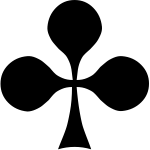
\includegraphics[width=0.4\textwidth]{_Klaveren.png}
\caption{Met natuurlijk een onderschrift.}
\label{fig:klaveren}%en een label
\end{figure}
Graag \verb|width=x\textwidth| gebruiken ipv \verb|scale=y|. Mooi hè, figuur \ref{fig:klaveren}?
\section{Bayes rule classification}
asdf
\section{Perceptron algorithm}
asdf
\section{Model checking with existing software}
asdf
\begin{thebibliography}{x}
\bibitem{asdf}...and so is this reference!
\end{thebibliography}
\appendix
\section{Code}
=rand(200,99)
\end{document}
